\documentclass{article}
\usepackage{graphicx}
\usepackage[margin=1.5cm]{geometry}
\usepackage{amsmath}
\usepackage{fancyvrb}
\usepackage{url}

\begin{document}

\title{Synopsis - Week 13 Integrated Project: Hardware Acceleration}
\author{Prof. Jordan C. Hanson}

\maketitle

\section{Finite Impulse Response (FIR) Filter}

\noindent
A finite impulse response (FIR) filter takes digitized data as the input, and returns modified data of the same shape as the output.  Let $n$ represent the number of samples of digitized data.  Let $x[n]$ represent the vector of digitized input data, and $y[n]$ represent the digitized output data.  Let $z^{-1}$ represent an operation that selects the prior sample, or the $n-1$ sample relative to sample $n$.  Let the coefficients $b_n$ multiply the samples $x[n]$ as they pass through an amplifier.  Finally, let $\Sigma$ represent an adder that sums to inputs and produces one output.  A generalized circuit diagram for the FIR filter is shown in Fig. \ref{fig:fir}, and the formula relating the input to the output is given in Eq. \ref{eq:fir}.

\begin{figure}[ht]
\centering
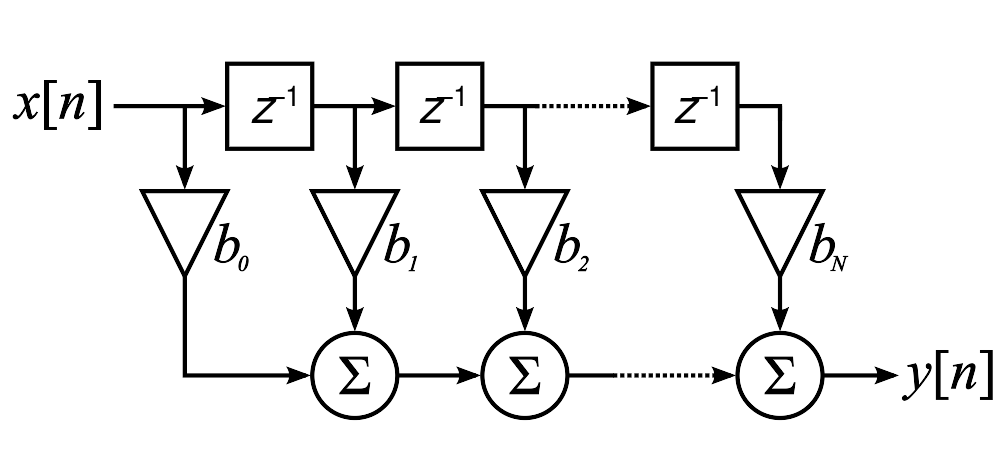
\includegraphics[width=0.33\textwidth]{figures/FIR_Filter.png}
\caption{\label{fig:fir} A generalized circuit diagram for the FIR filter.}
\end{figure}

\begin{equation}
y[n] = \sum_{i=0}^N b_i x[n-i]
\label{eq:fir}
\end{equation}

\noindent
In this lab, we are going to create a PYNQ overlay that will implement Eq. \ref{fig:fir} in the SoC PL layer.  We will show that:

\begin{itemize}
\item Implementing the FIR filter in the PL layer \textit{accelerates} the results
\item The acceleration depends on $N$, the number of data samples
\end{itemize}

\section{Example of an FIR Filter in SciPy}

Copy the following code into a Jupyter Notebook on the PYNQ-Z1 board:

\begin{verbatim}
import matplotlib.pyplot as plt
def plot_to_notebook(time_sec,in_signal,n_samples,out_signal=None):
    plt.figure()
    plt.subplot(1, 1, 1)
    plt.xlabel('Time (usec)')
    plt.grid()
    plt.plot(time_sec[:n_samples]*1e6,in_signal[:n_samples],'y-',label='Input signal')
    if out_signal is not None:
        plt.plot(time_sec[:n_samples]*1e6,out_signal[:n_samples],'g-',linewidth=2,label='FIR output')
    plt.legend()
\end{verbatim}

\noindent
This Python function will plot time samples in microseconds versus data samples in Volts.  If a second signal is given, it will be plotted with the same time samples.  The following code creates a list of time samples, sampled at 100 MHz, that is 1 ms long.  The result is $10^5$ samples.  There are $10^5$ samples because the \textit{sampling rate} is 100 million samples per second, for 1 ms.  The \verb+linspace+ function is used to create a list of $N = 10^5$ samples evenly spaced between 0 and 1 ms.

\begin{verbatim}
import numpy as np
# Total time
T = 0.001
# Sampling frequency
fs = 100e6
# Number of samples
n = int(T * fs)
# Time vector in seconds
t = np.linspace(0, T, n, endpoint=False)
# Samples of the signal
samples = 10000*np.sin(0.2e6*2*np.pi*t) + 1500*np.cos(46e6*2*np.pi*t) + 2000*np.sin(12e6*2*np.pi*t)
# Convert samples to 32-bit integers
samples = samples.astype(np.int32)
print('Number of samples: ',len(samples))
# Plot signal to the notebook
plot_to_notebook(t,samples,2000)
\end{verbatim}

\noindent
The signal samples are the sum of three sinusoidal functions, with frequencies 0.2 MHz, 46 MHz, and 12 MHz.  The plot shows a noisy sine wave.  Our goal is to filter the higher frequencies, leaving just the first signal at 0.2 MHz.  Let $V_{\rm in}$ be the input amplitude in Volts, and $V_{\rm out}$ be the output amplitude in Volts.  Filtering the higher frequencies means we must use a \textit{low-pass filter}.  It follows that $P_{\rm in} \propto V^2_{\rm in}$, and $P_{\rm out} \propto V^2_{\rm out}$.  Let the \textit{gain} of a filter in decibels be

\begin{align}
G_{\rm dB} &= 20 \log_{10}\left( \frac{V_{\rm out}}{V_{\rm in}} \right) \\
G_{\rm dB} &= 10 \log_{10}\left( \frac{P_{\rm out}}{P_{\rm in}} \right)
\end{align}

\noindent
The gain versus frequency of our FIR low-pass filter is shown in Fig. \ref{fig:fir}.  Notice that 0 dB means the input and output have the same amplitude and power.  A gain of -3 dB implies the output power is half that of the input.

\begin{figure}[hb]
\centering
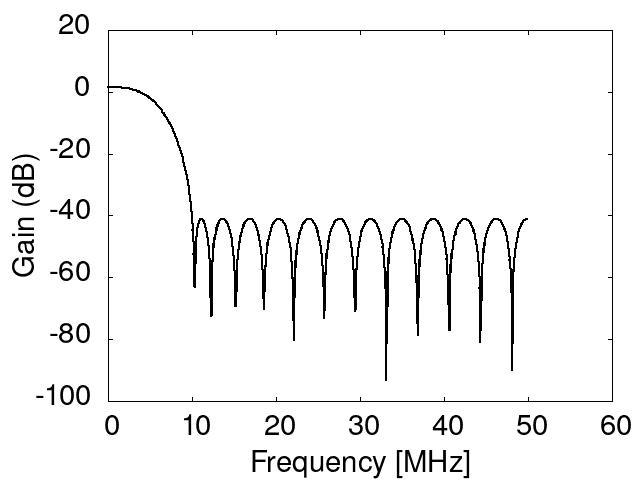
\includegraphics[width=0.5\textwidth]{FIR_gain_vs_freq.png}
\caption{\label{fig:fir} The gain in dB versus frequency of the FIR low-pass filter we will use in this lab activity.}
\end{figure}

\begin{enumerate}
\item What will happen to our signal, composed of three amplitudes at the three frequencies 0.2 MHz, 12 MHz, and 46 MHz, when it is passed through our FIR low-pass filter? \\ \vspace{1cm}
\item If we pass a 1 Volt, 20 MHz signal through our FIR low-pass filter, what will the final amplitude be in (a) dB (according to Fig. \ref{fig:fir}), and (b) in Volts? \\ \vspace{1cm}
\end{enumerate}

\noindent
The following code implements the FIR low-pass filter in Python.  Copy this code into your notebook for execution.  Make note of the SciPy function \verb+lfilter+ that implements Eq. \ref{eq:fir} with the coefficients $b_i$ given by the array \verb+coeffs+.

\begin{verbatim}
from scipy.signal import lfilter
import time
coeffs = [-255,-260,-312,-288,-144,153,616,1233,1963,2739,3474,4081,4481,4620,4481,4081,3474,2739,
1963,1233,616,153,-144,-288,-312,-260,-255]
start_time = time.time()
sw_fir_output = lfilter(coeffs,100e3,samples)
stop_time = time.time()
sw_exec_time = stop_time - start_time
print('Software FIR execution time: ',sw_exec_time)
# Plot the result to notebook
plot_to_notebook(t,samples,2000,out_signal=sw_fir_output)
\end{verbatim}

\noindent
Notice the execution time of the \verb+lfilter+ function is recorded in the variable \verb+sw_exec_time+.  What is a typical execution time for the \verb+lfilter+ function.  How does it appear to scale with $N$, the total number of samples?

\section{Creating a Block Diagram in Vivado with FIR Filter and DMA}

On the ASUS laptop, open the application \textit{Vivado} using the menu at the bottom left of the desktop environment.  Create a new project by choosing a project name and ensuring that it is an RTL (register-transfer level) project.  In the Default part dialogue, choose the Boards tab, then search for the PYNQ-Z1 board.  Select the PYNQ-Z1 board, then click Finish.  The screen should now resemble Fig. \ref{fig:vid_1}.  Locate the IP Integrator section on the left-hand column.  Click IP Integrator, and click OK in pop-up window named Create Block Design.  Using this functionality, we are going to add some digital logic to the standard PYNQ-Z1 PL.  In the diagram space, click the $+$ button, search for Zynq (the Xilinx SoC that powers the PYNQ-Z1).  Add the Zynq system to the diagram, which should resemble \ref{fig:vid_2} below.  Notice the bar at the top of the block diagram inviting the user to run block automation.  Run this to set the normal initial conditions to the Zynq block.

\begin{figure}
\centering
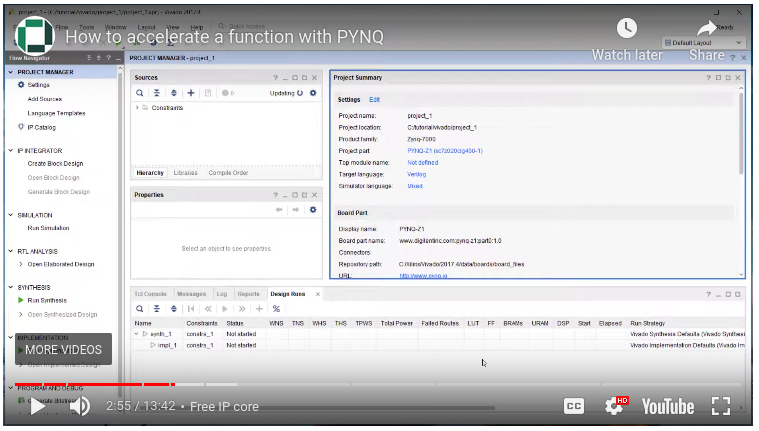
\includegraphics[width=0.45\textwidth]{fir_video_1.png}
\caption{\label{fig:vid_1} Beginning a firmware project in Vivado.}
\end{figure}

\begin{figure}[hb]
\centering
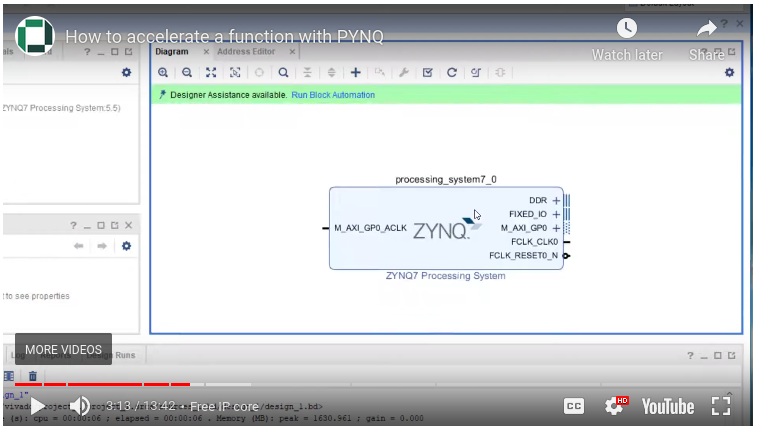
\includegraphics[width=0.45\textwidth]{fir_video_2.png}
\caption{\label{fig:vid_2} Adding the Zynq SoC to the block diagram.}
\end{figure}

\clearpage

\noindent
At the top of the block diagram, click the $+$ button and search for FIR Compiler.  Once the FIR block is added to the block diagram, double click it to open its settings.  Configure the FIR Compiler in the following ways:

\begin{enumerate}
\item Copy the \verb+coeffs+ list from the Jupyter notebook to the Coefficient Vector field in the FIR Compiler.
\item Click the Channel Specification tab, and under Hardware Oversampling Specification, set the input sampling frequency to 100 MHz.
\item Just below the sampling frequency, set the clock frequency to 100 MHz.  This will set the FIR filter to accept one new sample per clock cycle.
\item Click the Implementation tab, and scroll down to Data Path Options.  Set the input and output data widths to be 32 bits, just as they are generated in the Python3 code.  Set output rounding mode to ``non-symmetric rounding up.''  Full-precision output is not possible with 32 bit samples as inputs.
\item Under the Interface tab, select Packet Framing for TLAST, and check the Output Ready box.  These choices will help transfer the data between the PS and PL layers.
\item To finalize the FIR configuration, click OK.  The block diagram should now resemble Fig. \ref{fig:vid_3} (left).
\end{enumerate}

\begin{figure}
\centering
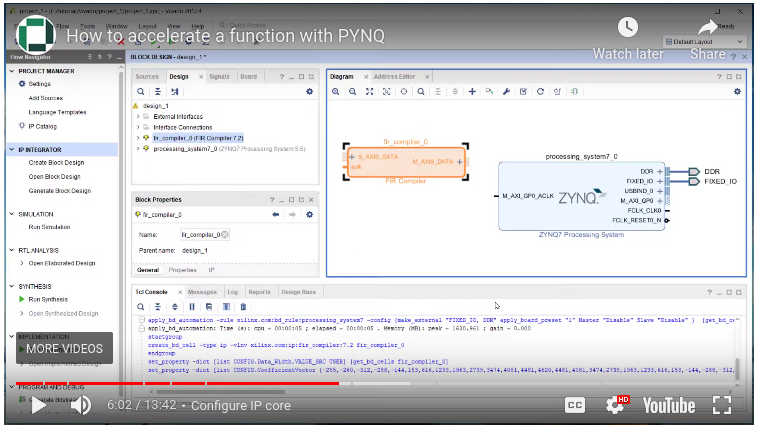
\includegraphics[width=0.45\textwidth]{fir_video_3.png}
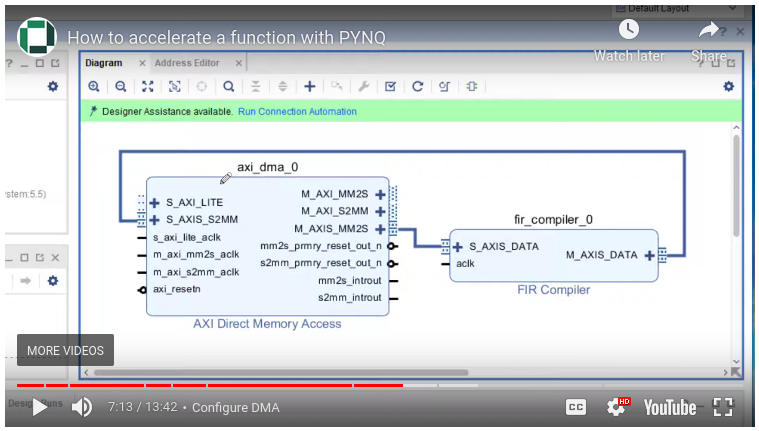
\includegraphics[width=0.45\textwidth]{fir_video_4.png}
\caption{\label{fig:vid_3} (Left) Adding the FIR filter block. (Right) Connections between DMA and FIR filter.}
\end{figure}

\noindent
The next IP component we will add is a direct memory access (DMA) block.  We need to find the input signal data by address in our Zynq system, pass it to the configured FIR filter, and pass the output back to the Zynq.  The DMA will manage this.  To add the DMA, click $+$ in the block diagram, and search for DMA.  Choose AXI Direct Memory Access, and wait for the new block to appear in our design.  Double click on the DMA block to configure it.  Perform the following tasks:

\begin{enumerate}
\item Disable ``scatter gather engine,'' (not supported in PYNQ-Z1).
\item Set the width of buffer length register to 23 bits.  This was the maximum when this project was created.  Click OK.
\end{enumerate}

\noindent
Now connect the proper outputs and inputs between the DMA and the FIR filter, as shown in Fig. \ref{fig:vid_3} (right).  Double click the Zynq block, and enable a high-performance AXI port by clicking the green block (bottom right of the diagram).

\begin{figure}[hb]
\centering
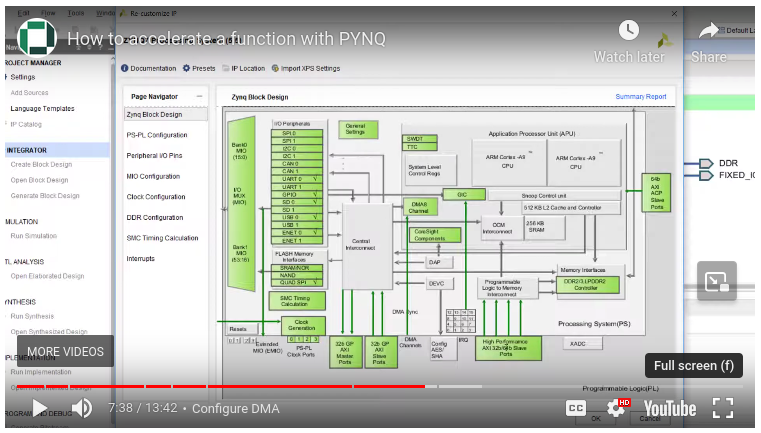
\includegraphics[width=0.45\textwidth]{fir_video_5.png}
\caption{\label{fig:vid_4} The inner workings of the Zynq SoC.}
\end{figure}

\clearpage

\noindent
Under PS-PL Configuration, enable ``S AXI HP0 interface.''  Click OK, and leave the Zynq block selected.  Now we can run connection automation via the green bar above the overall block diagram.  In the ensuing dialogue, check the boxes for the AXI DMA, FIR Compiler, and processing system connections.  Vivado will discern which connections make sense in light of the usual functionality of these blocks.  Click OK to run the automation.  Run the automation again, and leave the boxes checked.  The full block diagram should now resemble Fig. \ref{fig:vid_5}.  Click the DMA block, then under Block Properties, enter \verb+fir_dma+ in the Name field.  Similarly, re-name the FIR block \verb+fir+.  Select both the DMA and the FIR blocks by clicking one, then holding \verb+Shift+ key, and clicking the second.  Right-click the pair of blocks and select Create Hierarchy.  Name the hierarchy filter.  This will make the new PL easier to reference in Python3.  Save the block design by clicking the disk icon at the top left of the Vivado window.

\begin{figure}
\centering
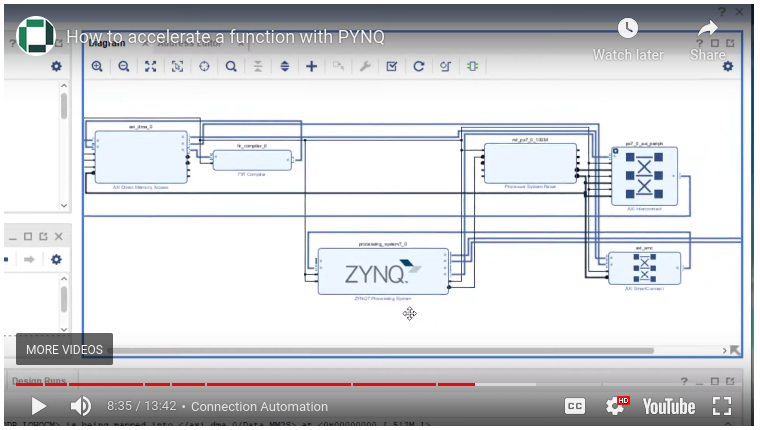
\includegraphics[width=0.45\textwidth]{fir_video_6.png}
\caption{\label{fig:vid_5} The inner workings of the Zynq SoC.}
\end{figure}

\section{Creating a Custom PYNQ Overlay}

Locate the pane with Design, Sources, Signals, and Board tabs.  Click Sources, and under Design Sources, right-click on the design file \verb+design_1+.  Select create HDL wrapper, and click OK in the pop-up window.  When this process is finished, locate the Program and Debug section in the left pane.  Click generate bitstream.  Click OK until the process begins.  Using the HDL wrapper, this should generate the \verb+.bit+ file that will be loaded by the PYNQ-Z1 SoC as an ``overlay.''  The overlay will keep all of the original SoC functionality, and add the FIR filter logic function.  When the bitstream is generated, go to \verb+File+, \verb+Export+, and export the block design to a TCL file.  Give your TCL file the name \verb+fir_accel.tcl+.  Now open a file browser on the laptop, and accomplish these three remaining tasks:
\begin{enumerate}
\item In the project folder corresponding the design, find and rename the HDL wrapper \verb+fir_accel.bit+.
\item Similarly, locate the ``hardware handoff'' file (.hwh), and rename it \verb+fir_accel.hwh+.
\item Gather together \verb+fir_accel.bit+, \verb+fir_accel.tcl+, and \verb+fir_accel.hwh+ in the Downloads folder of Linux.
\end{enumerate}

\noindent
We must now mv the files to the right location on our PYNQ-Z1 board.  Return to the browser that corresponds to the PYNQ-Z1 system.  Using the Upload button at the top right, load the files onto the board.  We must then put them in the right location.  Follow these steps to do this:
\begin{enumerate}
\item In the browser, open a terminal (New $\rightarrow$ Terminal), for interacting with the operating system.
\item Type \verb+pwd+.  This command prints the working directory, or current directory.
\item Notice we are in the \verb+root+ directory, or $/$.  Type \verb+cd /home/xilinx/jupyter_notebooks+, then type \verb+ls+.
\item Do you see the files named \verb+fir_accel.bit+, \verb+fir_accel.tcl+, and \verb+fir_accel.hwh+? 
\item The \verb+mv+ (move) command works like: \verb+mv file /path/to/destination/+.
\item Using the \verb+mv+ command, move the files to \verb+/home/xilinx/pynq/overlays+.
\item Now change directories (cd) like \verb+cd /home/xilinx/pynq/overlays+.
\item Create a directory called \verb+fir_accel+ using the \verb+mkdir+ command: \verb+mkdir fir_accel+.
\item Move the files into the \verb+fir_accel+ directory.
\end{enumerate}

\clearpage

\section{Using the FIR Low-Pass Filter in the PL Layer}

The \verb+pynq+ package \verb+Overlay+ loads bit files.  We usually load the \verb+base.bit+ for our lab activities involving \verb+logictools+.  Execute the code below to load our new bitstream, and gain access to the DMA block.

\begin{verbatim}
from pynq import Overlay
import pynq.lib.dma
# Load the overlay
overlay = Overlay('/home/xilinx/pynq/overlays/fir_accel/fir_accel.bit')
# Load the FIR DMA
dma = overlay.filter.fir_dma
\end{verbatim}

\noindent
The final code block below performs several actions.  First, we need the \verb+allocate+ function to copy (bit by bit) the 32-bit data samples into correctly-shaped ``buffers'' that will be fed through the DMA to the FIR filter in the PL layer. The buffers need to know $N$, the number of samples.  The functions from the \verb+time+ package will time the operations.  It is important to count the data transfer time as well as time required to filter the data.  The DMA sub-classes \verb+sendchannel+ and \verb+recvchannel+ are the inputs and outputs, and the \verb+transfer+ function moves the data accordingly.  The \verb+out_buffer+ receives the filtered data.  We calculate the ratio of the ``software execution time'' and the ``hardware execution time'' to find the ``speed-up factor.''  Finally, we plot some samples of the un-filtered and filtered data from \verb+out_buffer+, and free the \verb+in_buffer+ and \verb+out_buffer+ memory.

\begin{verbatim}
from pynq import allocate
import numpy as np
# Allocate buffers for the input and output signals
in_buffer = allocate(shape=(n,), dtype=np.int32)
out_buffer = allocate(shape=(n,), dtype=np.int32)
# Copy the samples to the in_buffer
np.copyto(in_buffer,samples)
# Trigger the DMA transfer and wait for the result
import time
start_time = time.time()
dma.sendchannel.transfer(in_buffer)
dma.recvchannel.transfer(out_buffer)
dma.sendchannel.wait()
dma.recvchannel.wait()
stop_time = time.time()
hw_exec_time = stop_time-start_time
print('Hardware FIR execution time: ',hw_exec_time)
print('Hardware acceleration factor: ',sw_exec_time / hw_exec_time)
# Plot to the notebook
plot_to_notebook(t,samples,1000,out_signal=out_buffer)
# Free the buffers
in_buffer.close()
out_buffer.close()
\end{verbatim}

\section{Measuring Speed-Up Factor vs. $N$}

Determine how the speed-up factor depends on $N$, the number of samples.  Measure the speed-up factor several times for each new $N$ value you choose, so that you can obtain an average.  Plot the average speed-up factor versus $N$.  Try plotting speed-up versus $\log_{10}(N)$.  Do you notice the trend?

\end{document}
